\section{Il nuovo modello}

\begin{frame}
	\frametitle{La funzione di interazione spaziale}
	\centering
	
	\begin{columns}[T]
		
		\begin{column}[t]{0.48\linewidth}
			\textbf{Espressione}
			\begin{equation*}
				h_\rho(\mathbf{s}|\mathcal{S}) = \left(1 + \sum_{\mathbf{s}^\prime\in\mathcal{S}}f_\rho(\mathbf{s}, \mathbf{s}^\prime)\right)^{-1}
			\end{equation*}
			\begin{equation*}
				f_\rho(\mathbf{s}, \mathbf{s}^\prime) = f(\| \mathbf{s} - \mathbf{s}^\prime \|) = \text{exp}\left(-\frac{\|\mathbf{s} - \mathbf{s}^\prime\|}{\rho}\right)
			\end{equation*}
			\justifying
			dove $\mathcal{S}$ è l'insieme degli $N$ punti spaziali nei quali è stata misurata la variabile d'interesse.
		\end{column}
		
		\begin{column}{.02\textwidth}
			\rule{.1mm}{0.7\textheight}
		\end{column}
	
		\begin{column}[t]{0.48\linewidth}
			\textbf{Limiti}
			\begin{equation*}
				\lim\limits_{\rho\to 0} f_\rho(\| \mathbf{s} - \mathbf{s}^\prime \|) = 0
			\end{equation*}
			\begin{equation*}
				\lim\limits_{\rho\to 0} h_\rho(\mathbf{s}|\mathcal{S}) = 1
			\end{equation*}
			\begin{equation*}
				\lim\limits_{\rho\to\infty} f_\rho(\| \mathbf{s} - \mathbf{s}^\prime \|) = 1
			\end{equation*}
			\begin{equation*}
				\lim\limits_{\rho\to\infty} h_\rho(\mathbf{s}|\mathcal{S}) = \frac{1}{N+1}
			\end{equation*}
		\end{column}
	\end{columns}
\end{frame}

\begin{frame}
	\frametitle{Il Functional Potential Hidden Dynamic Geostatistical Model (fp-HDGM)}
	\centering
	\begin{equation*}
		y(\mathbf{s}, l, t|\mathcal{S}) = w(\mathbf{s}, l, t)\cdot\textcolor{red}{h_\rho(\mathbf{s}|\mathcal{S})}
	\end{equation*}
	\begin{equation*}
		w(\mathbf{s}, l, t) = \mathbf{x}(\mathbf{s}, l, t)^\top\cdot\boldsymbol{\beta}(l) + \Phi_z(l)^\top\cdot \mathbf{z}(\mathbf{s}, t) + \epsilon(\mathbf{s}, l, t)
	\end{equation*}
	\begin{equation*}
		z(\mathbf{s}, t) = G\cdot\mathbf{z}(\mathbf{s}, t-1) + \boldsymbol{\eta}(\mathbf{s}, t)
	\end{equation*}
	\newline
	\justifying
	dove $\textcolor{red}{h_\rho(\mathbf{s}|\mathcal{S})}$ condiziona le osservazioni $w(\mathbf{s}, l, t)$ prive della componente interattiva e modellate utilizzando il modello f-HDGM. \textcolor{red}{$\rho$} è il nuovo parametro da stimare, il quale descrive l'intensità dell'interazione spaziale.
\end{frame}

\begin{frame}
	\frametitle{Simulazione di una mappa di potenziale al variare di $\rho$}
	
	\begin{columns}[T]
		\begin{column}[t]{0.5\linewidth}
			\centering
			$\rho = 0$
			\begin{figure}
				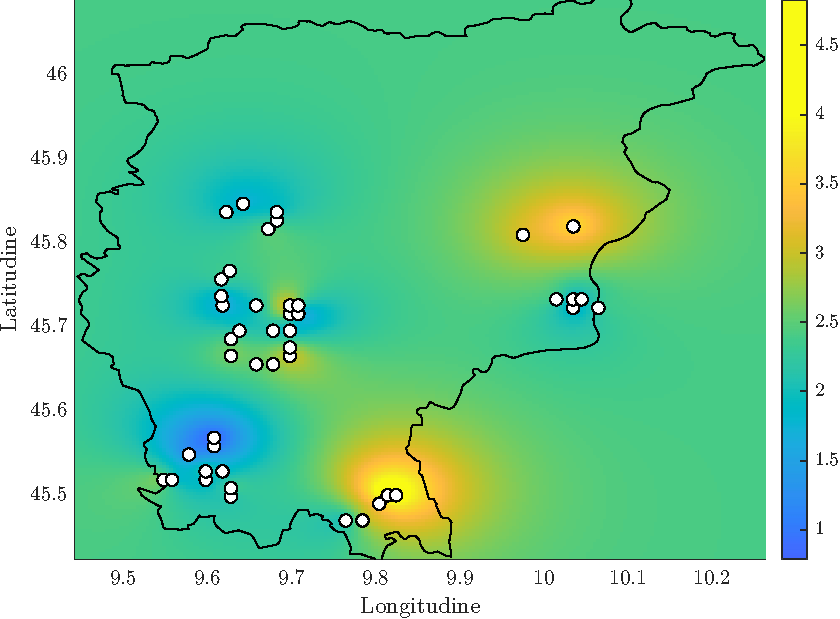
\includegraphics[width=\textwidth]{../Tesi/Immagini/2. Nuovo modello/Mappa potenziale, rho = 0}
			\end{figure}
		\end{column}
		\begin{column}[t]{0.5\linewidth}
			\centering
			$\rho = 0.5\cdot 10^{-2}$
			\begin{figure}
				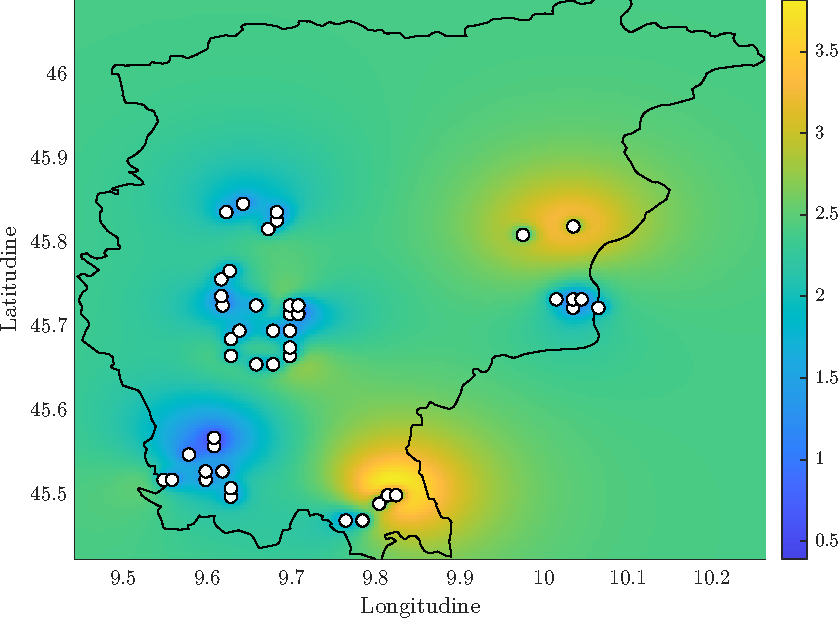
\includegraphics[width=\textwidth]{../Tesi/Immagini/2. Nuovo modello/Mappa potenziale, rho = 0.005}
			\end{figure}
		\end{column}
	\end{columns}

\end{frame}

\begin{frame}
	
	\begin{columns}[T]
		\begin{column}[t]{0.5\linewidth}
			\centering
			$\rho = 10^{-2}$
			\begin{figure}
				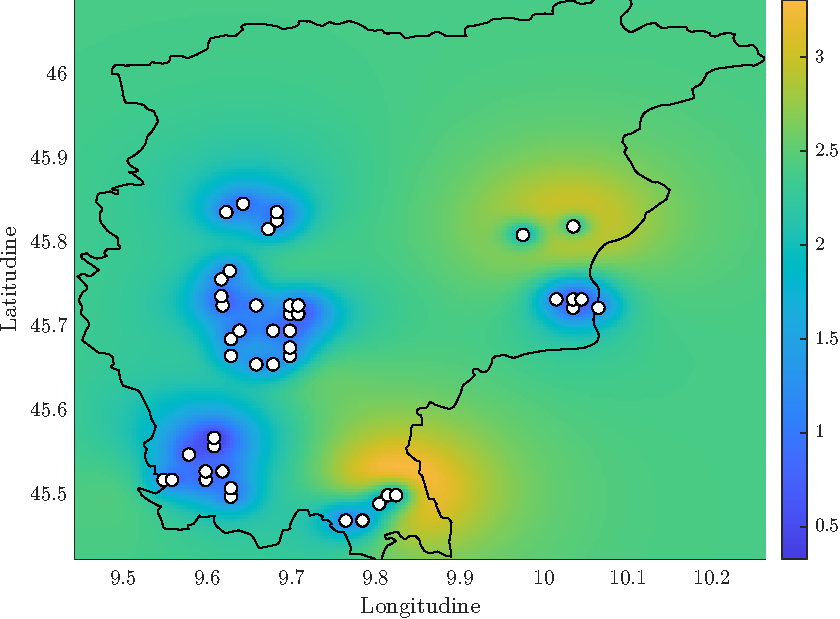
\includegraphics[width=\textwidth]{../Tesi/Immagini/2. Nuovo modello/Mappa potenziale, rho = 0.01}
			\end{figure}
		\end{column}
		\begin{column}[t]{0.5\linewidth}
			\centering
			$\rho = 1.5\cdot 10^{-2}$
			\begin{figure}
				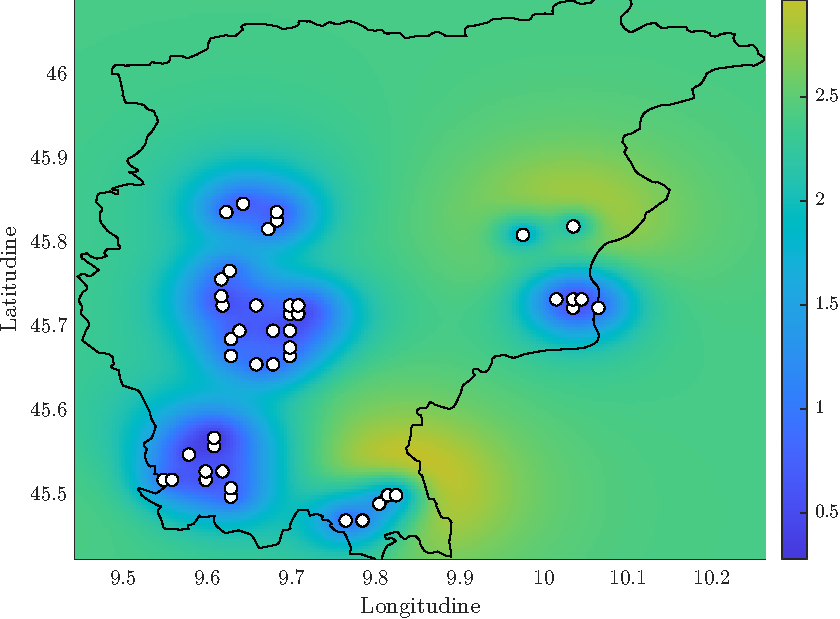
\includegraphics[width=\textwidth]{../Tesi/Immagini/2. Nuovo modello/Mappa potenziale, rho = 0.015}
			\end{figure}
		\end{column}
	\end{columns}
	
\end{frame}